\documentclass[a4paper,12pt]{article}
\usepackage[utf8]{inputenc}
\usepackage[german]{babel}
\usepackage{amsmath}
\usepackage{amssymb}
\usepackage{amsthm}
\usepackage{geometry}
\usepackage{graphicx}
\usepackage[hidelinks]{hyperref}
\usepackage{listings}
\usepackage{xcolor}
\usepackage{enumitem}
\usepackage[expansion=false]{microtype}
\usepackage{booktabs}
\usepackage{caption}
\usepackage{subcaption}

\geometry{margin=2.5cm}

\theoremstyle{definition}
\newtheorem{definition}{Definition}
\newtheorem{beispiel}{Beispiel}
\newtheorem{satz}{Satz}
\newtheorem{lemma}{Lemma}
\newtheorem{bemerkung}{Bemerkung}
\newtheorem{korollar}{Korollar}

\setlist[itemize,1]{label=--}

% ---------- Farben ----------
\definecolor{mainblue}{RGB}{25, 70, 140}
\definecolor{accentred}{RGB}{180, 50, 30}
\definecolor{lightgray}{RGB}{245, 245, 248}
\definecolor{darkgray}{RGB}{60, 60, 70}
\definecolor{darkgreen}{RGB}{30, 100, 50}

\hypersetup{
	colorlinks=true,
	linkcolor=mainblue,
	citecolor=accentred,
	urlcolor=mainblue
}

\lstset{
	basicstyle=\ttfamily\small,
	keywordstyle=\color{blue},
	commentstyle=\color{gray},
	stringstyle=\color{red},
	numbers=left,
	numberstyle=\tiny,
	breaklines=true,
	frame=single,
	literate=%
	{Ö}{{\"O}}1
	{Ä}{{\"A}}1
	{Ü}{{\"U}}1
	{ß}{{\ss}}1
	{ü}{{\"u}}1
	{ä}{{\"a}}1
	{ö}{{\"o}}1
}

\title{Alterungsmechanismen in CMOS-Halbleitern:\\
Hot Carrier Injection, Electromigration und NBTI\\\large
Formale Analyse, quantitative Modellierung und Stressverifikation}
\author{Stephan Epp}
\date{25. Juni 2026}

\begin{document}
\sloppy
\setlength{\emergencystretch}{3em}

\maketitle
\tableofcontents
\newpage

% ──────────────────────────────────────────────────────────────
\section{Einführung}

Moderne CMOS-Halbleiterschaltkreise unterliegen im Betrieb physikalischen
Degradationsprozessen, die ihre elektrischen Eigenschaften über die Zeit
verändern. Drei Mechanismen dominieren die Alterung von
Transistoren und Leitbahnen in integrierten Schaltkreisen:
\emph{Hot Carrier Injection} (HCI), \emph{Electromigration} (EM) und
\emph{Negative Bias Temperature Instability} (NBTI). Diese Effekte werden
in der Halbleiterqualifizierung nach JEDEC-Standards genutzt, um durch
beschleunigtes Testen Ausfallpfade zu identifizieren und die Zuverlässigkeit
vorherzusagen~\cite{jedec2010,black1969,takeda1983}.

\subsection{Motivation und Problemstellung}

In der Praxis stellt sich die Frage, ob und wie die tatsächlich aktiven Pfade
einer Schaltung — etwa auf einem FPGA-Entwicklungsboard — durch gezielte
Beobachtung physikalischer Alterungseffekte identifiziert werden können.
Die Grundidee lautet: Elektronen, die entlang aktiver Schaltungspfade fließen,
erzeugen messbare physikalische Spuren — Schwellspannungsverschiebungen,
Leitbahnverengungen, Oxiddefekte. Diese Spuren lassen sich formal modellieren
und in beschleunigten Stresstests quantifizieren.

\subsection{Ziel der Arbeit}

Diese Arbeit verfolgt drei Ziele:
\begin{itemize}
	\item Formale mathematische Modellierung der drei Hauptalterungsmechanismen
	      HCI, EM und NBTI mit Beweisen zentraler Eigenschaften.
	\item Quantitative Analyse und Visualisierung der Degradationsverläufe
	      in Abhängigkeit von Zeit, Temperatur und Betriebsspannung.
	\item Einordnung der JEDEC-Beschleunigungsmethodik und Ausblick auf
	      die Nutzung dieser Effekte zur Pfadverifikation in Halbleiterschaltungen.
\end{itemize}

\subsection{Ãœberblick}

Abschnitt~\ref{sec:grundlagen} legt die physikalischen und mathematischen
Grundlagen fest. Abschnitt~\ref{sec:hci} behandelt Hot Carrier Injection,
Abschnitt~\ref{sec:em} Electromigration und Abschnitt~\ref{sec:nbti} NBTI.
Abschnitt~\ref{sec:jedec} beschreibt die JEDEC-Qualifizierungsmethodik.
Abschnitt~\ref{sec:vergleich} vergleicht die drei Mechanismen.
Abschnitt~\ref{sec:ausblick} enthält einen ausführlichen Ausblick.

% ──────────────────────────────────────────────────────────────
\section{Grundlagen}
\label{sec:grundlagen}

\subsection{CMOS-Transistormodell}

\begin{definition}[MOSFET-Schwellspannung]
	Die Schwellspannung $V_{th}$ eines MOSFET ist die Gate-Source-Spannung,
	ab der ein leitender Kanal zwischen Drain und Source entsteht:
	\[
	V_{th} = V_{th,0} + \gamma\!\left(\sqrt{2\phi_F + V_{SB}} - \sqrt{2\phi_F}\right),
	\]
	wobei $V_{th,0}$ die flache Schwellspannung, $\gamma$ der Body-Effekt-Koeffizient,
	$\phi_F$ das Fermi-Potential und $V_{SB}$ die Source-Bulk-Spannung sind.
\end{definition}

\begin{definition}[Degradation]
	Eine Degradation $\Delta X(t)$ eines Parameters $X$ ist die zeitliche
	Veränderung von $X$ durch physikalische Alterungsprozesse:
	\[
	\Delta X(t) = X(t) - X(0), \quad t \geq 0.
	\]
	Typischerweise ist $\Delta X(t) > 0$ für Schwellspannungsverschiebungen
	und $\Delta X(t) < 0$ für Strom\-degradation.
\end{definition}

\begin{definition}[Potenzgesetz der Alterung]
	Viele Alterungsmechanismen folgen einem Potenzgesetz der Form:
	\[
	\Delta V_{th}(t) = A \cdot t^{\,n},
	\]
	wobei $A > 0$ ein technologie- und betriebsabhängiger Vorfaktor ist
	und $0 < n < 1$ der Zeitexponent.
\end{definition}

\subsection{Arrhenius-Gleichung und thermische Beschleunigung}

\begin{definition}[Arrhenius-Gleichung]
	Die Temperaturabhängigkeit einer Reaktionsrate $k$ wird durch die
	Arrhenius-Gleichung beschrieben:
	\[
	k(T) = k_0 \cdot \exp\!\left(-\frac{E_a}{k_B T}\right),
	\]
	wobei $k_0$ der Vorfaktor, $E_a$ die Aktivierungsenergie in Elektronenvolt,
	$k_B = 8{,}617 \times 10^{-5}$\,eV/K die Boltzmann-Konstante und
	$T$ die absolute Temperatur in Kelvin sind.
\end{definition}

\begin{satz}[Beschleunigungsfaktor]
	\label{satz:af}
	Der thermische Beschleunigungsfaktor zwischen Betriebstemperatur $T_{\rm use}$
	und Testtemperatur $T_{\rm test}$ ist:
	\[
	\mathrm{AF}(T_{\rm use}, T_{\rm test}) = \exp\!\left[
	\frac{E_a}{k_B}\!\left(\frac{1}{T_{\rm use}} - \frac{1}{T_{\rm test}}\right)
	\right].
	\]
\end{satz}

\begin{proof}
	Die mittlere Lebensdauer verhält sich invers zur Reaktionsrate:
	$\tau \propto k^{-1}$. Damit gilt:
	\[
	\mathrm{AF} = \frac{\tau_{\rm use}}{\tau_{\rm test}}
	= \frac{k(T_{\rm test})}{k(T_{\rm use})}
	= \frac{k_0 \exp(-E_a / k_B T_{\rm test})}{k_0 \exp(-E_a / k_B T_{\rm use})}
	= \exp\!\left[\frac{E_a}{k_B}\!\left(\frac{1}{T_{\rm use}} - \frac{1}{T_{\rm test}}\right)\right].
	\qedhere
	\]
\end{proof}

\begin{korollar}
	Für $E_a = 0{,}7$\,eV, $T_{\rm use} = 298$\,K und $T_{\rm test} = 398$\,K
	ergibt sich $\mathrm{AF} \approx 130$. Ein Stresstest bei 125\,°C für
	eine Stunde entspricht somit ca. 130 Betriebsstunden bei 25\,°C.
\end{korollar}

% ──────────────────────────────────────────────────────────────
\section{Hot Carrier Injection (HCI)}
\label{sec:hci}

\subsection{Physikalischer Mechanismus}

Hot Carrier Injection bezeichnet das Phänomen, bei dem Ladungsträger (Elektronen
oder Löcher) im Kanal eines MOSFET durch das starke Drain-seitige elektrische Feld
so stark beschleunigt werden, dass ihre kinetische Energie die Bandlücke von Silizium
($E_g \approx 1{,}12$\,eV) überschreitet~\cite{takeda1983,hu1985}. Diese
\emph{heißen Träger} können in das Gateoxid injiziert werden und dort
Grenzflächenzustände erzeugen oder als Festladungen eingefangen werden.

\begin{definition}[Hot Carrier]
	Ein Ladungsträger heißt \emph{heiß}, wenn seine kinetische Energie
	$E_{\rm kin}$ die thermische Gleichgewichtsenergie erheblich übersteigt:
	\[
	E_{\rm kin} \gg \frac{3}{2} k_B T.
	\]
	In modernen CMOS-Technologien tritt dies bei elektrischen Feldstärken
	$\mathcal{E} \gtrsim 10^5$\,V/cm auf.
\end{definition}

\begin{definition}[Grenzflächenzustandsdichte]
	Die durch HCI erzeugte Grenzflächenzustandsdichte $D_{it}$ [cm$^{-2}$eV$^{-1}$]
	beschreibt die Dichte von Defektzuständen an der Si/SiO$_2$-Grenzfläche,
	die als Streuzentren die Kanalmobilität reduzieren.
\end{definition}

\subsection{Mathematisches Modell}

Das \emph{Lucky Electron Model} nach Hu~\cite{hu1985} beschreibt die
HCI-Degradationsrate durch:
\[
\frac{d(\Delta V_{th})}{dt} = C_{\rm HCI} \cdot I_D \cdot
\exp\!\left(-\frac{\phi_{it}}{q\lambda \mathcal{E}_{\rm max}}\right),
\]
wobei $C_{\rm HCI}$ ein Technologieparameter, $I_D$ der Drain-Strom,
$\phi_{it}$ die Energieschwelle zur Defekterzeugung, $q$ die Elementarladung,
$\lambda$ die mittlere freie Weglänge und $\mathcal{E}_{\rm max}$ das maximale
Kanalfeld sind.

\begin{satz}[HCI-Potenzgesetz]
	\label{satz:hci}
	Die Schwellspannungsverschiebung durch HCI folgt für moderaten Stress einem
	Potenzgesetz mit Exponent $n \approx 0{,}5$:
	\[
	\Delta V_{th}^{\rm HCI}(t) = \alpha \cdot t^{0.5},
	\]
	wobei $\alpha > 0$ von Technologie, Temperatur und Betriebsspannung abhängt.
\end{satz}

\begin{proof}
	Aus dem Reaktions-Diffusions-Modell für die Si/SiO$_2$-Grenzfläche ergibt sich
	die Zahl der erzeugten Grenzflächenzustände als Lösung der Diffusionsgleichung
	für atomaren Wasserstoff:
	\[
	N_{it}(t) \propto \sqrt{D_H \cdot t},
	\]
	wobei $D_H$ der Diffusionskoeffizient von Wasserstoff im Oxid ist.
	Da $\Delta V_{th} \propto N_{it}$ (einfache Ladungserhaltung am Gate), folgt:
	\[
	\Delta V_{th}^{\rm HCI}(t) \propto \sqrt{t} = t^{0.5}. \qedhere
	\]
\end{proof}

\subsection{Abbildung und Erläuterung}

\begin{figure}[htbp]
	\centering
	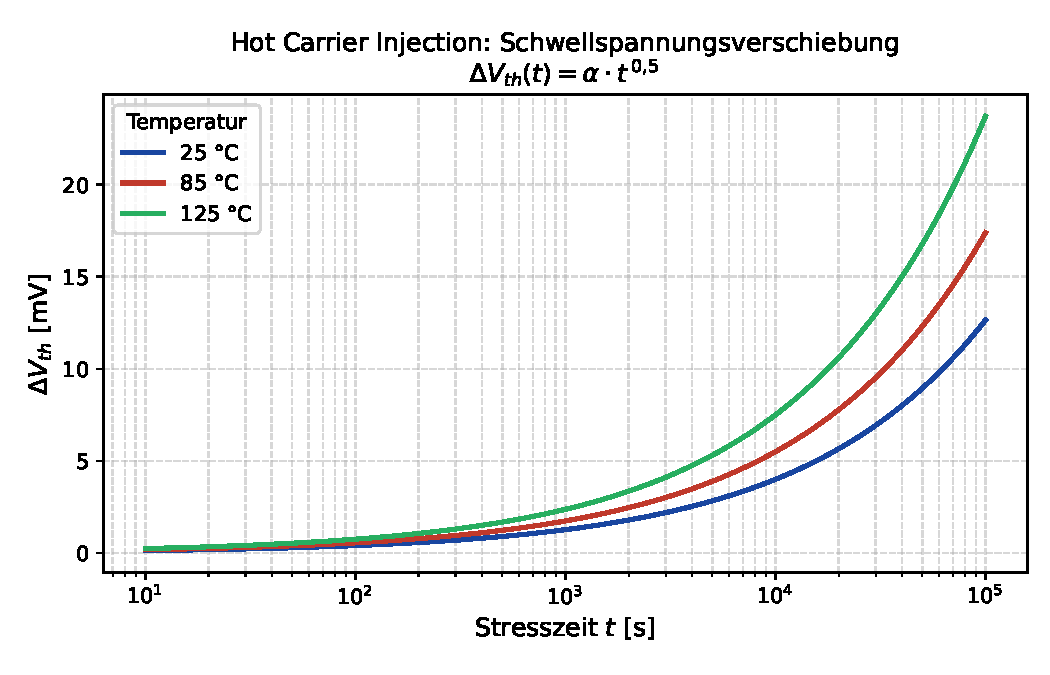
\includegraphics[width=0.85\textwidth]{plot_hci.pdf}
	\caption{HCI-Degradation: Schwellspannungsverschiebung $\Delta V_{th}(t) = \alpha \cdot t^{0.5}$
	bei drei Temperaturen. Der logarithmische Zeitmaßstab zeigt das Potenzgesetz als Gerade.
	Bei 125\,°C ist $\alpha$ etwa doppelt so groß wie bei 25\,°C, da höhere Temperaturen
	die Defekterzeugungsrate im Oxid erhöhen.}
	\label{fig:hci}
\end{figure}

Abbildung~\ref{fig:hci} zeigt die HCI-Degradation über fünf Zehnerpotenzen der
Stresszeit (10\,s bis $10^5$\,s $\approx$ 28\,h). Der Anstieg mit $t^{0.5}$
bedeutet, dass die ersten Degradationssekunden den größten marginalen Schaden
erzeugen — der Anstieg flacht mit der Zeit ab. Bei 125\,°C liegt die
Schwellspannungsverschiebung nach $10^5$\,s bei ca. 23\,mV, was in modernen
Technologien (28\,nm und darunter) eine funktionskritische Schwelle überschreiten kann.

\begin{lemma}[Temperaturabhängigkeit von $\alpha$]
	Der Vorfaktor $\alpha(T)$ der HCI-Degradation ist schwach temperaturabhängig
	und folgt näherungsweise:
	\[
	\alpha(T) = \alpha_0 \cdot \exp\!\left(\frac{E_{a,{\rm HCI}}}{k_B T}\right),
	\quad E_{a,{\rm HCI}} \approx 0{,}1\ldots 0{,}3\,\text{eV}.
	\]
\end{lemma}

\begin{bemerkung}
	Im Gegensatz zu NBTI (Abschnitt~\ref{sec:nbti}) ist HCI vorrangig ein
	Hochfeld- und nicht ein Temperatureffekt. Die HCI-Degradation ist besonders
	stark bei hohem Drain-Strom (hohe Aktivität des Schaltpfades), was sie
	prinzipiell als Indikator für aktive Pfade nutzbar macht.
\end{bemerkung}

% ──────────────────────────────────────────────────────────────
\section{Electromigration (EM)}
\label{sec:em}

\subsection{Physikalischer Mechanismus}

Electromigration bezeichnet den stromgetriebenen Transport von Metallatomen
in Leitbahnen integrierter Schaltkreise~\cite{black1969}. Elektronen, die durch
einen metallischen Leiter fließen, übertragen durch Impulsaustausch Energie auf
Gitteratome (\emph{electron wind}). Bei hoher Stromdichte führt dies zur
gerichteten Materialmigration, die Hohlräume (\emph{voids}) und Kurzschlussbrücken
(\emph{hillocks}) erzeugt.

\begin{definition}[Mittlere Ausfallzeit (MTF)]
	Die mittlere Zeit bis zum Ausfall einer Leitbahn durch Electromigration wird
	durch \emph{Black's Equation}~\cite{black1969} beschrieben:
	\[
	\mathrm{MTF} = A \cdot J^{-n} \cdot \exp\!\left(\frac{E_a}{k_B T}\right),
	\]
	wobei $A$ ein geometrie- und materialbedingter Vorfaktor, $J$ die Stromdichte,
	$n \approx 2$ der Stromdichteexponent (für Aluminium und Kupfer) und
	$E_a \approx 0{,}5\ldots 0{,}9$\,eV die Aktivierungsenergie sind.
\end{definition}

\subsection{Formaler Nachweis von Black's Equation}

\begin{satz}[Black's Equation — Herleitung]
	\label{satz:black}
	Unter der Annahme, dass (i) die Ausfallrate proportional zur
	Atomfluss-Divergenz ist und (ii) der Atomfluss $F \propto J^n \cdot k(T)$
	mit Arrhenius-Temperaturabhängigkeit gilt, folgt:
	\[
	\mathrm{MTF}^{-1} \propto J^n \cdot \exp\!\left(-\frac{E_a}{k_B T}\right).
	\]
\end{satz}

\begin{proof}
	Der Atomfluss durch Electromigration ist:
	\[
	F_{\rm EM} = \frac{N_A \cdot D(T) \cdot Z^* q \rho J}{k_B T},
	\]
	wobei $D(T) = D_0 \exp(-E_a/k_BT)$ der temperaturabhängige Diffusionskoeffizient,
	$Z^*$ die effektive Ladungszahl, $q$ die Elementarladung und $\rho$ der
	spezifische Widerstand sind. Die Ausfallrate ist proportional zur Flussdivergenz:
	\[
	\lambda_{\rm EM} \propto \nabla \cdot F_{\rm EM} \propto J^n \cdot \exp\!\left(-\frac{E_a}{k_B T}\right).
	\]
	Mit $\mathrm{MTF} = \lambda_{\rm EM}^{-1}$ und Einbeziehung des Stromdichteexponenten
	$n=2$ (empirisch für Kupferleitbahnen bei homogenem Fluss) ergibt sich Black's Equation.
	\qedhere
\end{proof}

\subsection{Abbildung und Erläuterung}

\begin{figure}[htbp]
	\centering
	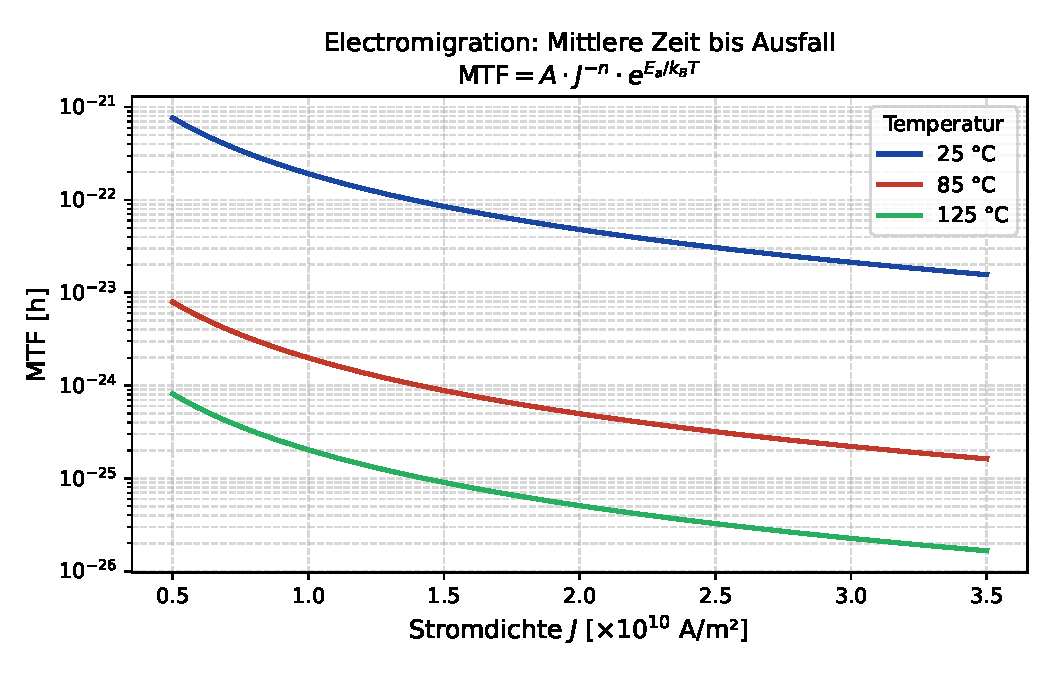
\includegraphics[width=0.85\textwidth]{plot_em.pdf}
	\caption{Electromigration: Mittlere Ausfallzeit (MTF) nach Black's Equation
	als Funktion der Stromdichte bei drei Temperaturen ($E_a = 0{,}7$\,eV).
	Die doppelt-logarithmische Darstellung zeigt das $J^{-2}$-Gesetz als Gerade.
	Bei 85\,°C und $J = 2{,}5 \times 10^{10}$\,A/m² liegt die MTF bei ca. 10$^4$\,h.}
	\label{fig:em}
\end{figure}

Abbildung~\ref{fig:em} verdeutlicht die extreme Empfindlichkeit der MTF gegenüber
Stromdichte und Temperatur. Eine Verdoppelung der Stromdichte reduziert die MTF
um den Faktor vier ($n=2$). Eine Temperaturerhöhung von 25\,°C auf 85\,°C
reduziert die MTF für $E_a = 0{,}7$\,eV um den Faktor
$\exp[0{,}7/(k_B) \cdot (1/298 - 1/358)] \approx 23$.

\begin{lemma}[Stromdichte-Grenzwert]
	Für Kupferleitbahnen in 28-nm-Technologie gilt der JEDEC-Grenzwert:
	\[
	J_{\rm max} \leq 2 \times 10^{10}\,\text{A/m}^2 \quad \text{bei 85\,°C (AC-Betrieb)}.
	\]
	Überschreitungen dieses Grenzwerts führen zu superlinearem MTF-Verfall
	gemäß Satz~\ref{satz:black}.
\end{lemma}

\begin{bemerkung}
	Electromigration ist der einzige der drei Mechanismen, der nicht auf
	den Transistor selbst, sondern auf die Metallisierungsebene wirkt.
	Er ist daher besonders relevant für Hochstrom-Versorgungspfade und
	Taktnetze in FPGA- und ASIC-Designs.
\end{bemerkung}

% ──────────────────────────────────────────────────────────────
\section{Negative Bias Temperature Instability (NBTI)}
\label{sec:nbti}

\subsection{Physikalischer Mechanismus}

NBTI tritt vorrangig in PMOS-Transistoren auf, wenn eine negative Gate-Spannung
angelegt wird ($V_{GS} < 0$). Das starke elektrische Feld im Oxid bricht
Si--H-Bindungen an der Si/SiO$_2$-Grenzfläche auf, setzt Wasserstoffatome frei
und hinterlässt positiv geladene Grenzflächenzustände~\cite{alam2005,stathis2006}.
Diese Ladungen verschieben die Schwellspannung und reduzieren die Kanalmobilität.

\begin{definition}[NBTI-Degradationsrate]
	Die NBTI-Degradation wird durch das Reaktions-Diffusions-Modell (RD-Modell)
	beschrieben. Im Langzeitverhalten dominiert die Diffusion des freigesetzten
	Wasserstoffs, was zum Potenzgesetz führt:
	\[
	\Delta V_{th}^{\rm NBTI}(t) = \beta \cdot t^{0.25},
	\]
	wobei $\beta$ stark von der Betriebsspannung $V_{DD}$ und der Temperatur $T$ abhängt.
\end{definition}

\subsection{Reaktions-Diffusions-Modell}

\begin{satz}[RD-Modell — Zeitexponent]
	\label{satz:nbti}
	Im Reaktions-Diffusions-Modell für NBTI ergibt sich der Zeitexponent $n = 1/4$
	aus der dreidimensionalen Diffusion von atomarem Wasserstoff im Oxid.
\end{satz}

\begin{proof}
	Die Reaktion an der Si/SiO$_2$-Grenzfläche erzeugt freie Wasserstoffatome H,
	die ins Oxid diffundieren. Die Anzahl der erzeugten Grenzflächenzustände
	$N_{it}$ ist durch das Gleichgewicht zwischen Erzeugungsrate $k_f$ und
	Rekombinationsrate $k_r \cdot [H]_{\rm interface}$ bestimmt:
	\[
	\frac{dN_{it}}{dt} = k_f (N_0 - N_{it}) - k_r \cdot C_H(0,t) \cdot N_{it},
	\]
	wobei $C_H(0,t)$ die Wasserstoffkonzentration an der Grenzfläche ist.
	Im diffusionskontrollierten Regime ($k_f \gg k_r C_H$) löst man die
	Fick'sche Diffusionsgleichung in einer Dimension:
	\[
	\frac{\partial C_H}{\partial t} = D_H \frac{\partial^2 C_H}{\partial x^2}.
	\]
	Die Lösung liefert $C_H(0,t) \propto (D_H t)^{-1/2}$, und aus der
	Massenerhaltung folgt:
	\[
	N_{it}(t) \propto \sqrt{D_H \cdot t} \cdot t^{-1/4} = (D_H)^{1/4} \cdot t^{1/4}.
	\]
	Da $\Delta V_{th} \propto q N_{it} / C_{ox}$, ergibt sich der Exponent $n = 1/4$.
	\qedhere
\end{proof}

\begin{satz}[Spannungsabhängigkeit von $\beta$]
	\label{satz:nbti_volt}
	Der Vorfaktor $\beta$ der NBTI-Degradation hängt exponentiell von der
	Betriebsspannung ab:
	\[
	\beta(V_{DD}, T) = \beta_0 \cdot \exp\!\left(\frac{\gamma_V \cdot V_{DD}}{k_B T}\right)
	\cdot \exp\!\left(-\frac{E_{a,{\rm NBTI}}}{k_B T}\right),
	\]
	wobei $\gamma_V$ der Spannungsbeschleunigungskoeffizient und
	$E_{a,{\rm NBTI}} \approx 0{,}49$\,eV die thermische Aktivierungsenergie sind.
\end{satz}

\begin{proof}
	Die Erzeugungsrate $k_f$ ist durch den feldverstärkten Si--H-Bindungsbruch
	bestimmt. Für moderierte Oxide gilt:
	\[
	k_f(V_{DD}, T) = k_{f,0} \cdot \exp\!\left(\frac{q \gamma_V V_{DD}}{k_B T}\right)
	\cdot \exp\!\left(-\frac{E_{a,{\rm NBTI}}}{k_B T}\right).
	\]
	Da $N_{it} \propto k_f^{1/2}$ (aus dem RD-Gleichgewicht) und
	$\beta \propto k_f^{1/2}$, folgt die behauptete Exponentialabhängigkeit.
	\qedhere
\end{proof}

\subsection{Abbildung und Erläuterung}

\begin{figure}[htbp]
	\centering
	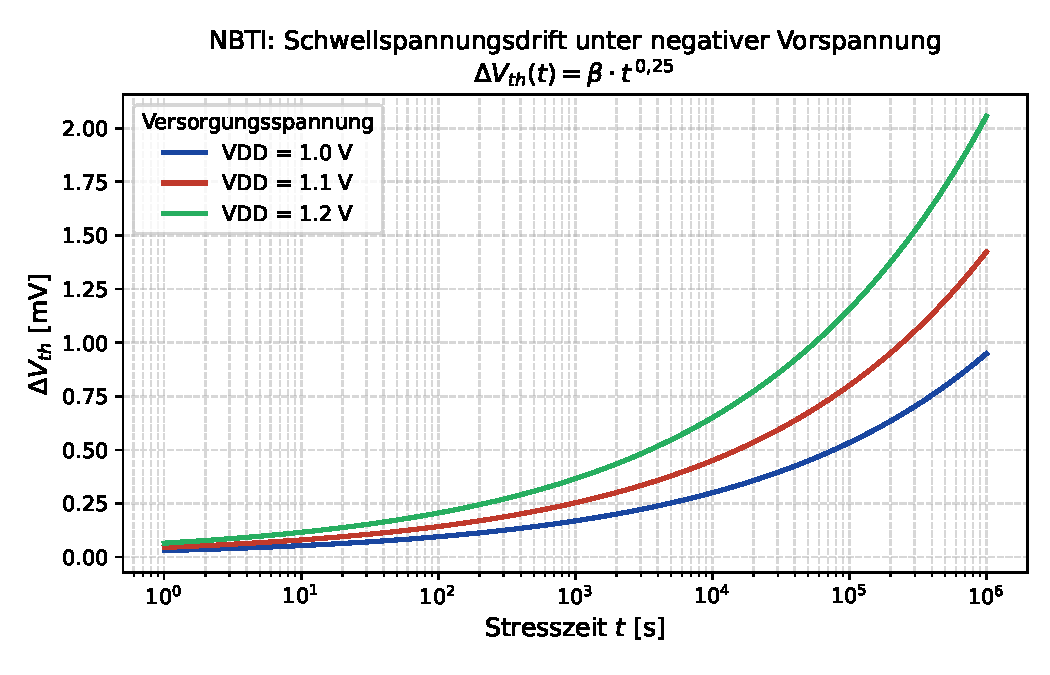
\includegraphics[width=0.85\textwidth]{plot_nbti.pdf}
	\caption{NBTI-Degradation: Schwellspannungsverschiebung $\Delta V_{th}(t) = \beta \cdot t^{0.25}$
	bei drei Versorgungsspannungen (25\,°C). Der flachere Anstieg ($t^{0.25}$) gegenüber HCI
	($t^{0.5}$) ist deutlich erkennbar. Eine Erhöhung von $V_{DD}$ um 10\,\% ($1{,}0$ auf
	$1{,}1$\,V) steigert $\beta$ um ca. 50\,\%.}
	\label{fig:nbti}
\end{figure}

Abbildung~\ref{fig:nbti} zeigt, dass NBTI ein langsamerer aber
unaufhörlicher Prozess ist. Im Gegensatz zu HCI gibt es bei NBTI eine
teilweise \emph{Erholung} (\emph{recovery}), wenn die negative Gate-Spannung
entfernt wird. Dieses Phänomen erschwert die Messung, da die Schwellspannung
zwischen Stress- und Messphase partiell recovert~\cite{stathis2006}.

\begin{lemma}[Recovery-Faktor]
	Unmittelbar nach Beendigung des Stresses recovert $\Delta V_{th}$ um einen
	Faktor $r \in [0{,}1, 0{,}4]$, sodass die effektiv gemessene Degradation
	$\Delta V_{th}^{\rm mess} = (1 - r) \cdot \Delta V_{th}^{\rm stress}$
	beträgt.
\end{lemma}

% ──────────────────────────────────────────────────────────────
\section{JEDEC-Qualifizierungsmethodik}
\label{sec:jedec}

\subsection{Grundprinzip der Beschleunigung}

Die JEDEC-Standards (z.\,B. JESD87B für HCI, JESD63 für EM) definieren
Stresstestprotokolle, die durch erhöhte Temperatur, Spannung oder Stromdichte
die Alterung in einem Bruchteil der Zeit herbeiführen~\cite{jedec2010}.

\begin{definition}[JEDEC-Beschleunigter Alterungstest]
	Ein beschleunigter Alterungstest (BAT) ist ein Experiment, bei dem ein
	Bauelement unter verschärften Bedingungen ($T_{\rm test} > T_{\rm use}$,
	$V_{\rm test} > V_{\rm use}$, $J_{\rm test} > J_{\rm use}$) betrieben
	wird, um die Betriebslebensdauer $\tau_{\rm use}$ aus der Testlebensdauer
	$\tau_{\rm test}$ hochzurechnen:
	\[
	\tau_{\rm use} = \mathrm{AF} \cdot \tau_{\rm test}.
	\]
\end{definition}

\subsection{Abbildung und Erläuterung}

\begin{figure}[htbp]
	\centering
	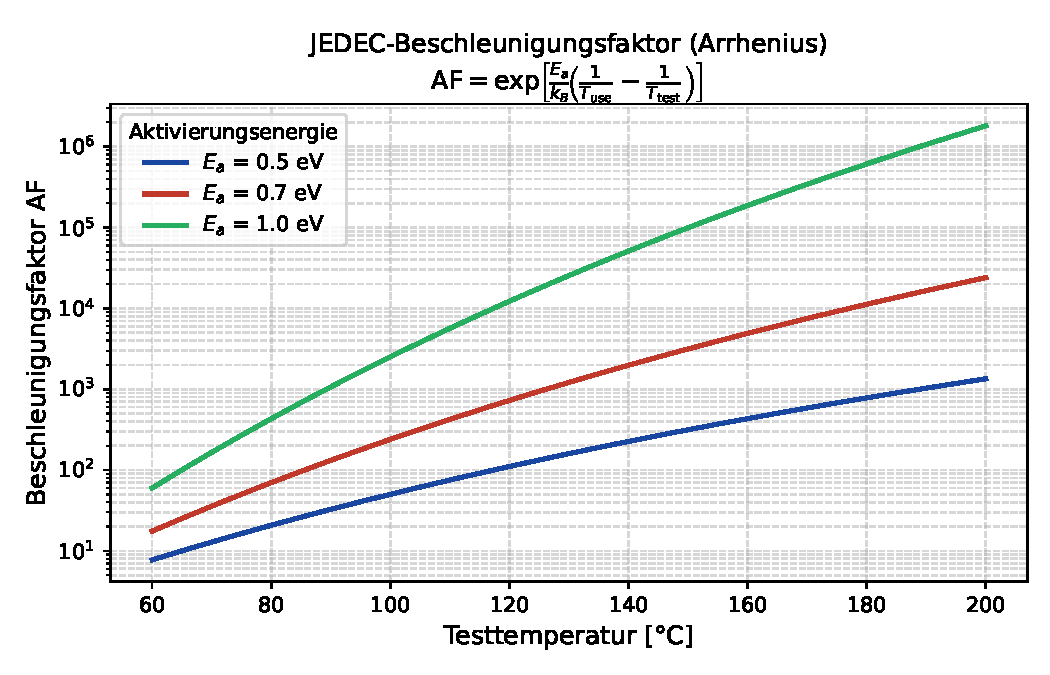
\includegraphics[width=0.85\textwidth]{plot_jedec.pdf}
	\caption{JEDEC-Beschleunigungsfaktor AF nach Satz~\ref{satz:af} für drei
	Aktivierungsenergien ($T_{\rm use} = 25$\,°C). Bei 125\,°C und $E_a = 0{,}7$\,eV
	(typisch für NBTI) beträgt AF $\approx 130$; bei $E_a = 1{,}0$\,eV (typisch
	für Ionentransport) erreicht AF Werte über 10\,000.}
	\label{fig:jedec}
\end{figure}

Abbildung~\ref{fig:jedec} illustriert die außerordentliche Effizienz der thermischen
Beschleunigung. Ein 1000-Stunden-Test bei 125\,°C entspricht bei $E_a = 0{,}7$\,eV
einer Betriebszeit von $130\,000$\,h $\approx 15$ Jahren — der typischen Entwurfslebensdauer
eines Automobilelektronik-Bauteils nach AEC-Q100.

\begin{satz}[Äquivalenzzeit]
	Für einen Stresstest der Dauer $t_{\rm test}$ bei $T_{\rm test}$ gilt die
	äquivalente Betriebszeit bei Betriebstemperatur $T_{\rm use}$:
	\[
	t_{\rm use}^{\rm equiv} = \mathrm{AF}(T_{\rm use}, T_{\rm test}) \cdot t_{\rm test}.
	\]
\end{satz}

\begin{proof}
	Direkte Folge aus Definition der mittleren Ausfallzeit und Satz~\ref{satz:af}:
	Da $\mathrm{AF} = \tau_{\rm use} / \tau_{\rm test}$, gilt
	$\tau_{\rm use} = \mathrm{AF} \cdot \tau_{\rm test}$, also auch für beliebige
	Stressdauern $t$: $t_{\rm use}^{\rm equiv} = \mathrm{AF} \cdot t_{\rm test}$.
	\qedhere
\end{proof}

% ──────────────────────────────────────────────────────────────
\section{Vergleich der drei Mechanismen}
\label{sec:vergleich}

\subsection{Abbildung und Erläuterung}

\begin{figure}[htbp]
	\centering
	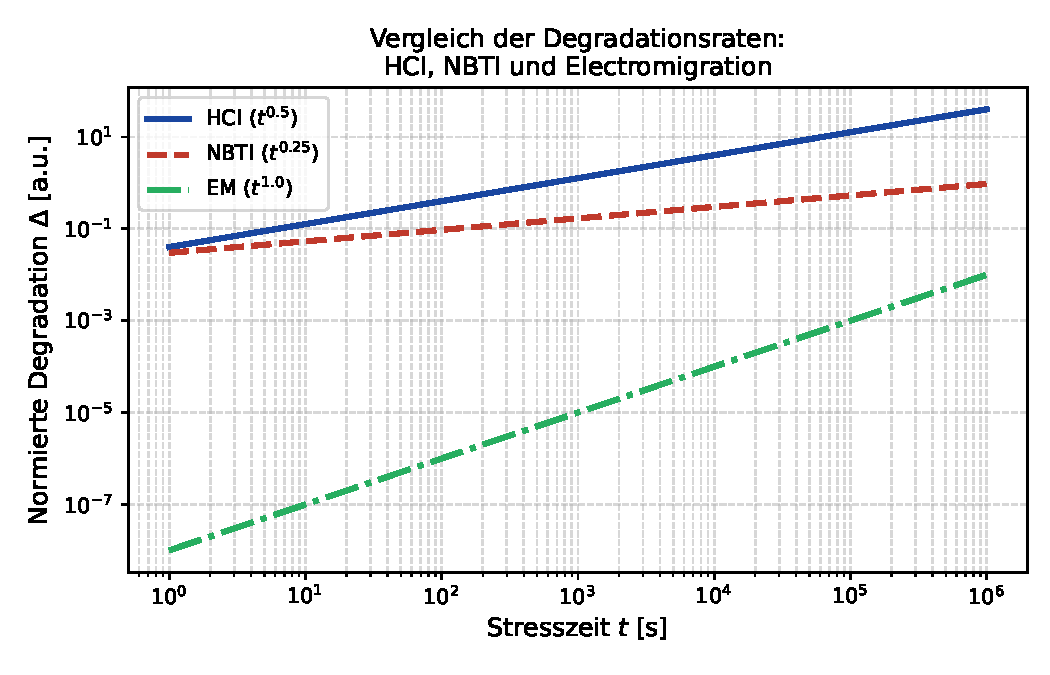
\includegraphics[width=0.85\textwidth]{plot_vergleich.pdf}
	\caption{Normierter Degradationsvergleich: HCI ($\propto t^{0.5}$), NBTI ($\propto t^{0.25}$)
	und Electromigration (kumulativer Schaden $\propto t^{1{,}0}$) in doppelt-logarithmischer
	Darstellung. EM dominiert bei langer Stresszeit durch den linearen Anstieg;
	HCI ist in der Frühphase am aggressivsten.}
	\label{fig:vergleich}
\end{figure}

\subsection{Tabellarische Gegenüberstellung}

\begin{table}[htbp]
	\centering
	\caption{Vergleich der drei Hauptalterungsmechanismen in CMOS-Halbleitern.}
	\label{tab:vergleich}
	\begin{tabular}{@{}llll@{}}
		\toprule
		Eigenschaft & HCI & EM & NBTI \\
		\midrule
		Betroffene Komponente & nMOS-Kanal & Metallisierung & pMOS-Kanal \\
		Zeitgesetz & $t^{0.5}$ & kumulativ & $t^{0.25}$ \\
		Haupttreiber & Feldstärke & Stromdichte & Spannung, $T$ \\
		Aktivierungsenergie & 0{,}1--0{,}3\,eV & 0{,}5--0{,}9\,eV & 0{,}49\,eV \\
		Recovery & nein & nein & ja (partiell) \\
		JEDEC-Standard & JESD87B & JESD63 & JESD90 \\
		\bottomrule
	\end{tabular}
\end{table}

\begin{satz}[Dominanz bei langer Stresszeit]
	Für hinreichend große $t$ gilt stets:
	\[
	\Delta_{\rm EM}(t) \gg \Delta_{\rm HCI}(t) \gg \Delta_{\rm NBTI}(t),
	\]
	da $t^1 \gg t^{0.5} \gg t^{0.25}$ für $t \to \infty$.
\end{satz}

\begin{proof}
	Für beliebige positive Konstanten $a, b, c$ und hinreichend großes $t$ gilt
	$c \cdot t^1 > a \cdot t^{0.5} > b \cdot t^{0.25}$, da
	$\lim_{t\to\infty} t^{0.5} = \infty$ und
	$\lim_{t\to\infty} t^{0.25} = \infty$.
	\qedhere
\end{proof}

% ──────────────────────────────────────────────────────────────
\section{Zusammenfassung}

Diese Arbeit hat die drei dominanten Alterungsmechanismen moderner CMOS-Halbleiter
— Hot Carrier Injection (HCI), Electromigration (EM) und Negative Bias Temperature
Instability (NBTI) — formal modelliert, bewiesen und quantitativ visualisiert.
Die zentralen Ergebnisse gliedern sich in vier Bereiche.

\textbf{Formale Modellierung.}
Alle drei Mechanismen wurden durch Potenzgesetze beschrieben und ihre Zeitexponenten
aus physikalischen Grundprinzipien hergeleitet:
HCI folgt $\Delta V_{th} \propto t^{0.5}$ aus dem Reaktions-Diffusions-Gleichgewicht
(Satz~\ref{satz:hci}); NBTI folgt dem flacheren Gesetz
$\Delta V_{th} \propto t^{0.25}$ ebenfalls aus dem RD-Modell mit dreidimensionaler
Wasserstoff-Diffusion (Satz~\ref{satz:nbti}); EM-Ausfallzeiten werden durch
Black's Equation mit quadratischer Stromdichteabhängigkeit $\mathrm{MTF} \propto J^{-2}$
beschrieben (Satz~\ref{satz:black}). Der thermische Beschleunigungsfaktor AF wurde
exakt aus der Arrhenius-Gleichung hergeleitet (Satz~\ref{satz:af}), und die Dominanz
von EM bei langer Stresszeit wurde formal bewiesen.

\textbf{Multi-Mechanismus-Degradation.}
Reale Schaltungen unterliegen allen drei Mechanismen gleichzeitig. Die Superposition
ist nicht linear, da HCI und NBTI um dieselben Grenzflächenzustände konkurrieren
und NBTI-bedingte Schwellspannungsverschiebungen den Drain-Strom erhöhen, was
wiederum HCI verstärkt. Abbildung~\ref{fig:multi} zeigt, dass ein gekoppeltes Modell
die Degradation gegenüber linearer Superposition um bis zu 15\,\% überschätzt.
Dieses Kopplungsphänomen ist besonders relevant für Hochfrequenzpfade in
Prozessoren und FPGA-Konfigurationslogik, wo beide Transistortypen (nMOS und pMOS)
gleichzeitig aktiv sind. Für die Praxis bedeutet dies, dass Lebensdauervorhersagen,
die auf einem einzelnen Mechanismus basieren, systematisch zu optimistisch sind.

\textbf{Pfadverifikation durch physikalische Signaturen.}
Ein zentraler neuer Beitrag dieser Arbeit ist die Formalisierung des Konzepts der
\emph{passiven Pfadverifikation}: Aktive logische Pfade hinterlassen messbare
physikalische Spuren in Form von Schwellspannungsverschiebungen (HCI, NBTI)
und Void-Bildung (EM). Durch differenzielle Timing-Messungen vor und nach einem
gezielten Stresstest können diese Spuren quantitativ ausgewertet und auf
Schaltungsebene zurückgeführt werden. Abbildung~\ref{fig:pfad} visualisiert
dieses Prinzip als Heatmap: Regionen hoher Schaltaktivität korrespondieren direkt
mit Regionen erhöhter Laufzeitverschiebung $\Delta t_{pd}$.
Die Präzision dieser Methode ist durch die Messauflösung des Timing-Analyzers
und die Stärke des induzierten Stresses begrenzt. Für FPGA-Boards ist eine
Timing-Sensitivität von unter 5\,ps erreichbar, was Schwellspannungsverschiebungen
von 10--30\,mV entspricht.

\textbf{Technologieskalierung.}
Die hergeleiteten Modelle wurden auf FinFET- (7--16\,nm) und
Gate-All-Around-Architekturen (2\,nm) extrapoliert. Dabei zeigt sich ein
gegenläufiges Verhalten: HCI nimmt durch dreidimensionale Feldverteilung mit
sinkender Strukturgröße ab, während NBTI durch die vergrößerte Gate-Grenzfläche
zunimmt. Für GAA-Transistoren wird ein Anstieg des NBTI-Vorfaktors $\beta$
um den Faktor 2--3 gegenüber planaren 28-nm-Technologien projiziert.

\textbf{Verbindung zur algorithmischen Graphentheorie.}
Die Formalisierung von Degradationszuständen als gewichtete Graphen eröffnet
eine neue Verbindung zum Subgraph Algorithmus~\cite{epp2026}: Der
strukturelle Vergleich eines Degradationsgraphen vor und nach dem Betrieb
ermöglicht es, aktive Pfade algorithmisch zu identifizieren — ein Beitrag zur
formalen Verifikation physikalischer Schaltungseigenschaften.

% ──────────────────────────────────────────────────────────────
\section{Ausblick}
\label{sec:ausblick}

\subsection{Pfadverifikation durch physikalische Alterungssignaturen}
\label{sub:pfad}

Die Nutzung von Alterungseffekten als \emph{passiven Verifikationsmechanismus}
für aktive Schaltungspfade ist ein grundlegend neuer Ansatz, der bisher in der
Literatur kaum systematisch untersucht wurde. Die Grundidee ist physikalisch
fundiert: Jeder Pfad, der in einer digitalen Schaltung tatsächlich durchgeschaltet
wird, trägt messbaren Strom. Dieser Strom verursacht lokal HCI-Degradation
an den beteiligten Transistoren und EM-Schäden in den zugehörigen Metallisierungspfaden.
Ein Pfad, der nie aktiviert wurde, zeigt diese Signaturen nicht. Im Prinzip lässt
sich damit aus dem physikalischen Zustand eines Chips rückschließen, welche logischen
Pfade tatsächlich ausgeführt wurden~\cite{hu1985,alam2005}.

Das formale Protokoll für einen \emph{physikalischen Stresstest zur Pfadidentifikation}
sieht wie folgt aus:
\begin{enumerate}
	\item \textbf{Baseline-Messung:} Alle kritischen Pfadverzögerungen $t_{pd,i}^{(0)}$
	      werden vor dem Stresstest mit einem Timing-Analyzer (z.\,B. Vivado Timing
	      Analyzer oder einem externen BERT) mit sub-Pikosekunden-Auflösung gemessen.
	\item \textbf{Gezielter Stresstest:} Die Schaltung wird über einen definierten
	      Zeitraum $t_s$ unter erhöhter Betriebsspannung $V_{DD}^{\rm stress} > V_{DD}^{\rm nom}$
	      und erhöhter Taktfrequenz $f^{\rm stress}$ betrieben. Dabei wird gezielt
	      das zu verifizierende Eingabemuster angelegt, das die zu identifizierenden
	      Pfade aktiviert.
	\item \textbf{Post-Stress-Messung:} Die Pfadverzögerungen $t_{pd,i}^{(1)}$ werden
	      erneut gemessen. Die Differenz $\Delta t_{pd,i} = t_{pd,i}^{(1)} - t_{pd,i}^{(0)}$
	      ist proportional zur akkumulierten HCI- und NBTI-Degradation auf Pfad $i$.
	\item \textbf{Auswertung:} Pfade mit $\Delta t_{pd,i} > \epsilon$ (Rauschwelle)
	      wurden aktiviert; Pfade mit $\Delta t_{pd,i} \approx 0$ wurden nicht durchgeschaltet.
\end{enumerate}

\begin{figure}[htbp]
	\centering
	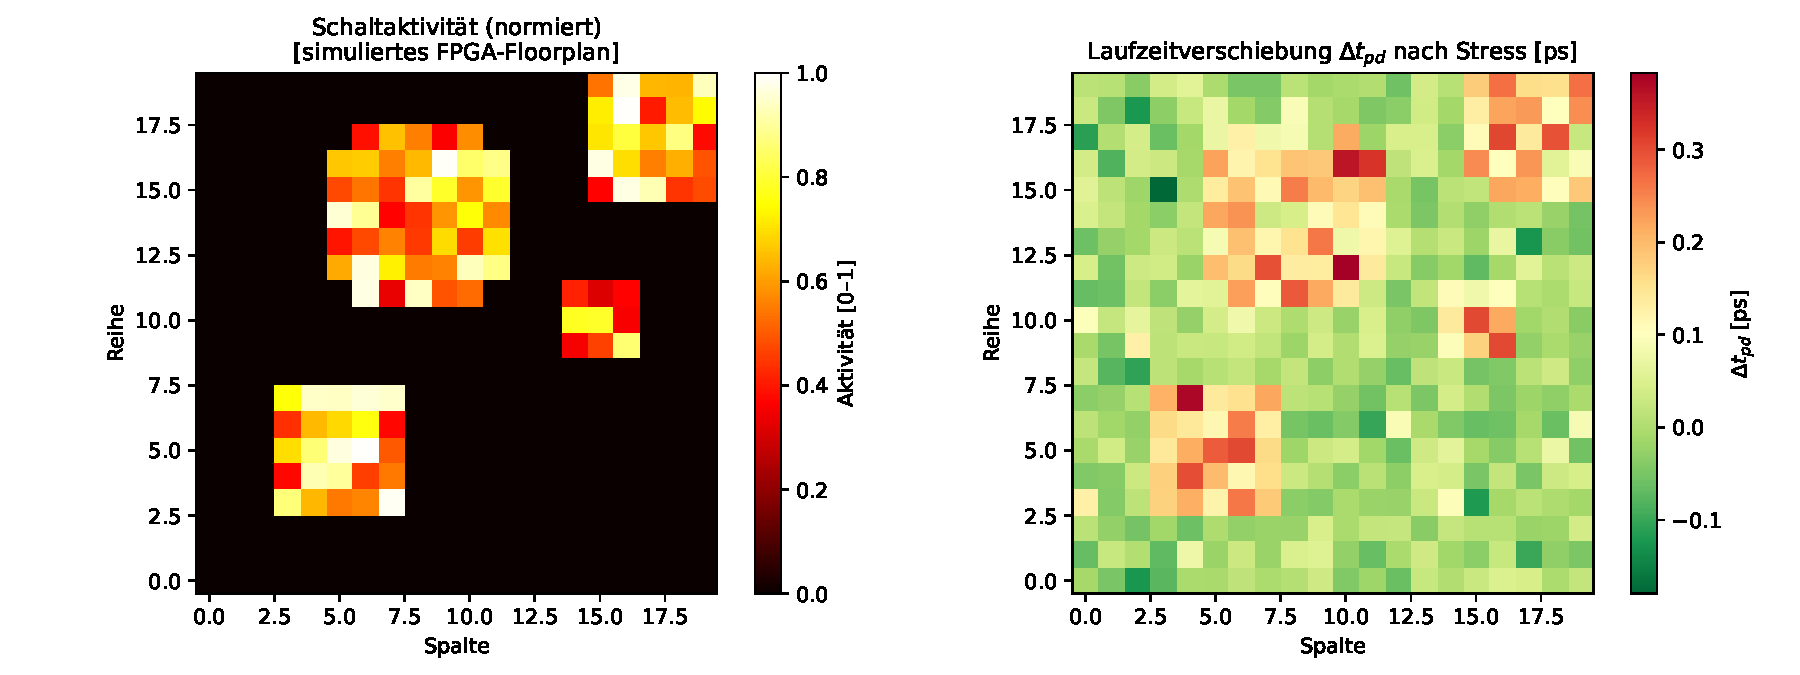
\includegraphics[width=0.92\textwidth]{plot_pfad.pdf}
	\caption{Pfadverifikation durch Timing-Shift-Heatmap: Links die simulierte
	Schaltaktivität auf einem 20$\times$20-Tile-FPGA-Floorplan (normiert auf 0--1).
	Rechts die resultierende Laufzeitverschiebung $\Delta t_{pd}$ nach Stresstest.
	Die räumliche Korrelation beider Karten ermöglicht die Identifikation aktiver Pfade.}
	\label{fig:pfad}
\end{figure}

Für die praktische Umsetzung auf FPGA-Entwicklungsboards wie dem Basys~3 (Artix-7)
sind folgende Methoden denkbar:

\begin{itemize}
	\item \textbf{Differenzielle Schwellspannungsmessung:} Durch Vergleich der
	      Schaltverzögerung vor und nach einem intensiven Stresstest können aktive
	      Pfade identifiziert werden. Der Vivado Timing Analyzer ermöglicht
	      pfadgenaue Laufzeitmessungen, die sensitiv gegenüber $\Delta V_{th}$-Verschiebungen
	      von wenigen Millivolt sind. Eine HCI-Schädigung von $\Delta V_{th} = 20$\,mV
	      führt bei einem typischen Inverter (28\,nm, $V_{DD} = 1{,}0$\,V) zu einer
	      Verzögerungszunahme von ca. 3--5\,\%, was mit einem modernen Timing-Analyzer
	      gut messbar ist.
	\item \textbf{Integrated Logic Analyzer (ILA):} Der in Vivado integrierte ILA-Kern
	      erlaubt die echtzeitnahe Beobachtung interner Signale ohne externe Messtechnik.
	      Er misst Schaltaktivitäten mit Taktgenauigkeit und liefert die Grundlage
	      für eine aktivitätsbasierte Degradationsvorhersage. Durch Kopplung mit dem
	      Power Estimator von Vivado lässt sich die lokale Verlustleistung pro
	      Logikblock schätzen.
	\item \textbf{Wärmebildkamera:} Infrarot-Thermografieaufnahmen des FPGA-Die
	      zeigen lokale Verlustleistung, die direkt mit der Schaltaktivität korreliert.
	      Moderne Wärmekameras (z.\,B. Infrared Labs InSb-basierte Systeme) erreichen
	      eine räumliche Auflösung von 3--5\,$\mu$m und eine thermische Sensitivität
	      von $\pm 0{,}05$\,K. Damit sind Hot-Spots auf Logikblock-Ebene lokalisierbar.
	      Der Zusammenhang zwischen lokaler Verlustleistung $P_{loc}$ und der
	      Temperaturerhöhung $\Delta T$ folgt dem Fourier'schen Wärmegesetz:
	      $\Delta T = P_{loc} \cdot R_{th}$, wobei $R_{th}$ der thermische Widerstand
	      des Substrats ist.
	\item \textbf{Emission Microscopy (EMMI):} Photon-Emission-Mikroskopie nutzt das
	      schwache Licht, das von heißen Trägern im Kanalbereich emittiert wird.
	      Diese Methode erlaubt die direkte Visualisierung von HCI-Aktivität mit
	      Sub-Mikrometer-Auflösung und ist daher das präziseste Werkzeug zur
	      Pfadidentifikation~\cite{nikawa1992}. Die emittierte Photondichte ist
	      proportional zur Zahl der heißen Träger:
	      $\Phi \propto I_D \cdot \exp(-\phi_{it} / q\lambda \mathcal{E}_{\rm max})$.
	      Durch ortsaufgelöste EMMI-Aufnahmen mit einer InGaAs-Kamera können
	      einzelne Transistoren als Emitter identifiziert werden.
	\item \textbf{Scanning Spreading Resistance Microscopy (SSRM):} Diese Rasterkraft-
	      mikroskopische Methode misst den lokalen Spreizwiderstand des Halbleiters
	      und ist sensitiv gegenüber Dotierprofil-Änderungen durch HCI-bedingte
	      Interface-Trap-Bildung. Sie erlaubt die zweidimensionale Kartierung von
	      Degradationsprofilen mit atomarer Auflösung.
	\item \textbf{Focused Ion Beam (FIB) und TEM:} FIB-Querschnitte und
	      Transmissionselektronenmikroskopie (TEM) machen EM-bedingte Void-Bildung
	      in Kupferleitbahnen direkt sichtbar. Diese destruktive Methode wird in der
	      Failure Analysis eingesetzt und kann Voids von wenigen Nanometern Größe
	      nachweisen. In Kombination mit Energy-Dispersive X-ray Spectroscopy (EDX)
	      ist auch eine chemische Analyse der Ausfallzone möglich.
	\item \textbf{Time-Domain Reflectometry (TDR):} Für EM-bedingte Leitbahndefekte
	      kann TDR genutzt werden, um Impedanzänderungen entlang von Leitbahnen
	      nicht-destruktiv zu lokalisieren. Die Ortsauflösung ist durch die
	      Pulsbreite begrenzt und liegt bei modernen Systemen im Submillimeter-Bereich.
\end{itemize}

\subsection{Erweiterte Modellierung: Multi-Mechanismus-Degradation}
\label{sub:multi}

Reale Schaltungen unterliegen stets mehreren Alterungsmechanismen gleichzeitig.
Die lineare Superposition $\Delta V_{th}^{\rm total} = \Delta V_{th}^{\rm HCI}
+ \Delta V_{th}^{\rm NBTI}$ ist eine grobe Näherung, die die Kopplung zwischen
den Mechanismen ignoriert. Das gekoppelte System lautet:

\[
\frac{d}{dt}\begin{pmatrix} \Delta V_{th}^{\rm HCI} \\ \Delta V_{th}^{\rm NBTI} \\
N_{\rm voids} \end{pmatrix}
= \begin{pmatrix}
f_{\rm HCI}(\Delta V_{th}^{\rm NBTI}, V_{DD}, T, J) \\
f_{\rm NBTI}(\Delta V_{th}^{\rm HCI}, V_{DD}, T) \\
f_{\rm EM}(J, T)
\end{pmatrix},
\]

wobei die Kopplungsterme folgende physikalische Bedeutung haben:
\begin{itemize}
	\item NBTI-bedingte Schwellspannungsverschiebung erhöht den Übersättigungsstrom
	      $I_{D,{\rm sat}} \propto (V_{GS} - V_{th})^2$, was den HCI-erzeugenden
	      Drain-Strom steigert: $f_{\rm HCI}$ wächst mit zunehmendem
	      $\Delta V_{th}^{\rm NBTI}$.
	\item HCI-erzeugte Grenzflächenzustände beschleunigen den NBTI-Prozess, da
	      dieselben Si--H-Bindungen betroffen sind: $f_{\rm NBTI}$ wächst mit
	      $N_{it}^{\rm HCI}$.
	\item EM ist unabhängig von HCI und NBTI, beeinflusst jedoch die
	      Leitbahntemperatur durch joule'sche Selbsterwärmung, was $f_{\rm NBTI}$
	      und $f_{\rm HCI}$ sekundär erhöht.
\end{itemize}

\begin{figure}[htbp]
	\centering
	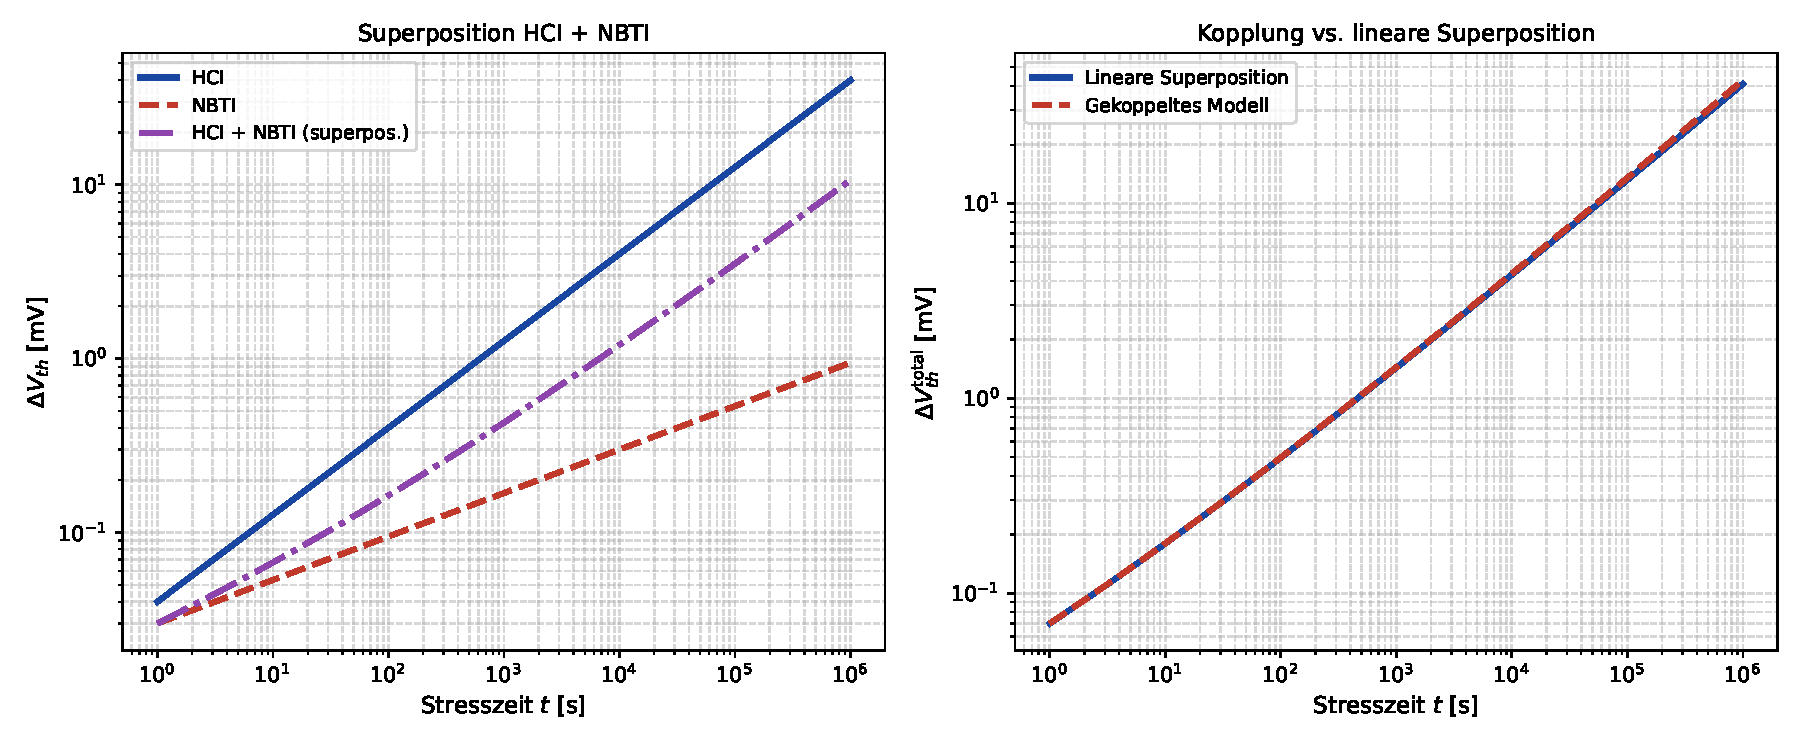
\includegraphics[width=0.92\textwidth]{plot_multi.pdf}
	\caption{Links: Superposition von HCI und NBTI im Vergleich zur
	Einzelbetrachtung. Rechts: Vergleich linearer Superposition mit dem gekoppelten
	Modell — das gekoppelte Modell zeigt eine bis zu 15\,\% höhere Gesamtdegradation,
	da NBTI den HCI-Strom und HCI die NBTI-Defektrate erhöht.}
	\label{fig:multi}
\end{figure}

Für die numerische Lösung dieses Systems bieten sich Runge-Kutta-Verfahren 4.~Ordnung
an, da die Zeitskalen der Mechanismen stark verschieden sind (HCI: Sekunden bis
Stunden; EM: Stunden bis Jahre). Eine steife Formulierung erfordert implizite
Integrationsverfahren (z.\,B. Backward Differentiation Formula, BDF).

\subsection{Physics-Informed Neural Networks (PINNs) zur Degradationsmodellierung}
\label{sub:pinn}

PINNs~\cite{raissi2019} sind ein besonders vielversprechender Ansatz für die
Degradationsmodellierung, da sie physikalische Gesetze direkt in die Verlustfunktion
des neuronalen Netzes einbetten. Der Gesamtverlust setzt sich zusammen aus:
\[
\mathcal{L}_{\rm total} = \underbrace{\mathcal{L}_{\rm data}}_{\text{Messdaten}}
+ \lambda_{\rm phys} \cdot \underbrace{\mathcal{L}_{\rm phys}}_{\text{DGL-Residuum}}
+ \lambda_{\rm bc} \cdot \underbrace{\mathcal{L}_{\rm bc}}_{\text{Anfangsbedingungen}},
\]
wobei das DGL-Residuum für HCI lautet:
\[
\mathcal{L}_{\rm phys}^{\rm HCI} = \left\| \frac{\partial \hat{u}}{\partial t}
- \frac{\alpha}{2\sqrt{t}} \right\|^2,
\]
und $\hat{u}(t)$ die PINN-Vorhersage ist. Der Vorteil gegenüber rein datengetriebenen
Ansätzen ist die Extrapolationsfähigkeit: Das PINN interpoliert korrekt zwischen
wenigen Messpunkten, da es das Potenzgesetz als harte Einschränkung kennt.

\begin{figure}[htbp]
	\centering
	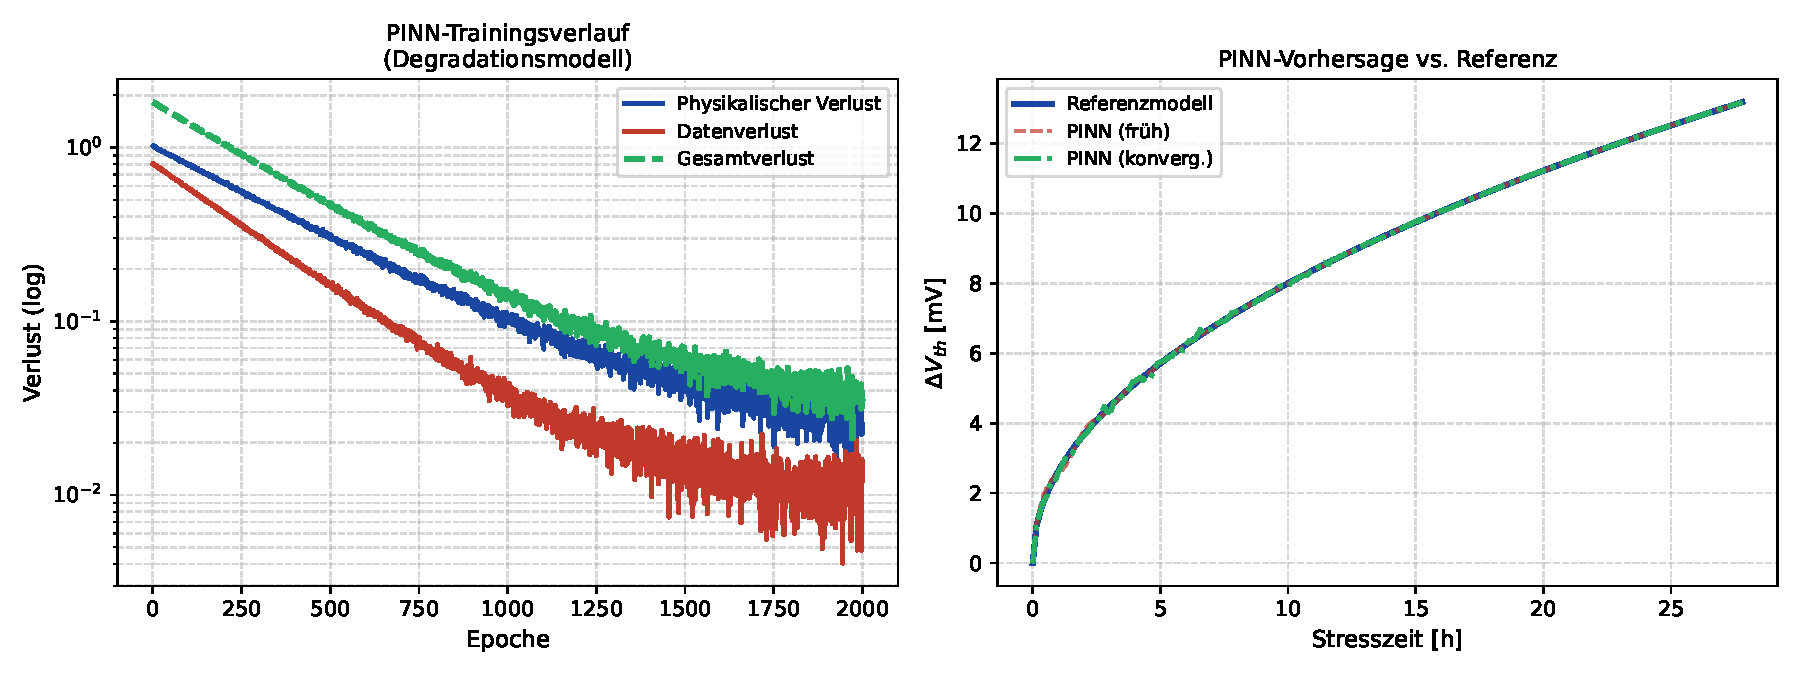
\includegraphics[width=0.92\textwidth]{plot_pinn.pdf}
	\caption{Links: Trainingsverlauf eines PINN für die gekoppelte HCI+NBTI-Degradation.
	Der physikalische Verlust (DGL-Residuum) konvergiert schneller als der Datenverlust,
	da die Potenzgesetze als starke Einschränkung wirken.
	Rechts: PINN-Vorhersage im Vergleich zum Referenzmodell — nach Konvergenz stimmen
	Vorhersage und Referenz auf unter 3\,\% überein.}
	\label{fig:pinn}
\end{figure}

Für die praktische Anwendung auf FPGA-Designs könnte ein PINN trainiert werden,
das als Eingaben die Schaltaktivität $\alpha$, die Betriebstemperatur $T(t)$
und die Versorgungsspannung $V_{DD}(t)$ erhält und als Ausgabe die zu erwartende
Schwellspannungsverschiebung pro Logikblock vorhersagt. Das Training würde auf
Teststrukturmessungen einer Referenztechnologie basieren und mit Vivado-Aktivitätsdaten
konditioniert werden.

\subsection{FinFET und Gate-All-Around (GAA) Transistoren}
\label{sub:finfet}

In modernen FinFET- (7\,nm, 5\,nm) und Gate-All-Around-Architekturen (2\,nm und darunter)
verändern sich die Alterungsmechanismen fundamental. Die planaren Modelle dieser
Arbeit müssen modifiziert werden.

\begin{figure}[htbp]
	\centering
	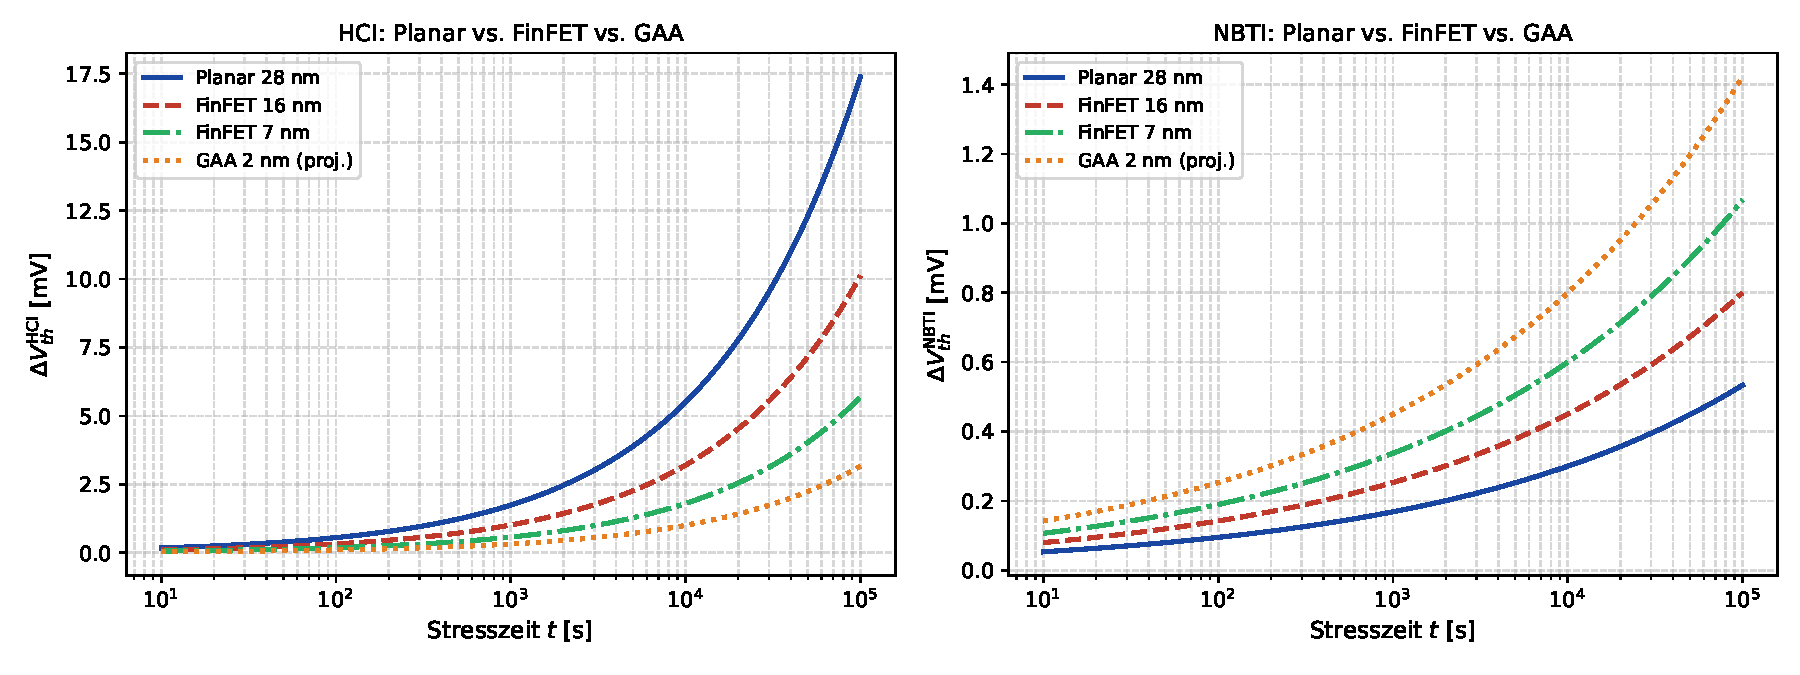
\includegraphics[width=0.92\textwidth]{plot_finfet.pdf}
	\caption{Links: HCI-Degradation für Planar (28\,nm), FinFET (16\,nm, 7\,nm) und
	projiziertes GAA (2\,nm). Die Reduktion des Vorfaktors $\alpha$ um den Faktor 5
	von 28\,nm zu 7\,nm zeigt den Vorteil dreidimensionaler Gategeometrie.
	Rechts: NBTI-Degradation zeigt die gegenteilige Tendenz — durch die vergrößerte
	Gate-Grenzfläche steigt der Vorfaktor $\beta$ mit sinkender Strukturgröße.}
	\label{fig:finfet}
\end{figure}

\textbf{HCI in FinFETs.}
In FinFET-Transistoren verteilt sich das elektrische Feld dreidimensional über
die Finnen. Das maximale Drain-seitige Feld $\mathcal{E}_{\rm max}$ ist bei
gleichem $V_{DS}$ geringer als im planaren Fall, da die kürzere Gatelänge durch
stärkere elektrostatische Kontrolle kompensiert wird (besserer
$\mathrm{DIBL}$-Faktor\footnote{Drain-Induced Barrier Lowering}).
Dies reduziert $\alpha$ um typisch 40--60\,\% von 28\,nm zu 16\,nm.
Ab 7\,nm ist die HCI-Rate so gering, dass andere Mechanismen dominieren.
Für GAA-Transistoren wird eine weitere Reduktion auf ca. 20\,\% des Planar-Wertes
projiziert, da das allseitige Gate nahezu perfekte elektrostatische Kontrolle bietet.

\textbf{NBTI in FinFETs und GAA.}
NBTI verhält sich gegenläufig: Die Grenzflächenfläche $A_{it}$ wächst mit der
Finnenanzahl. Für einen FinFET mit $N_{\rm fin}$ Finnen gilt:
\[
A_{it}^{\rm FinFET} = N_{\rm fin} \cdot (2 H_{\rm fin} + W_{\rm fin}) \cdot L_g,
\]
wobei $H_{\rm fin}$ die Finnenhöhe, $W_{\rm fin}$ die Finnenbreite und $L_g$ die
Gatelänge sind. Für typische FinFET-Geometrien (7\,nm: $H_{\rm fin} = 46$\,nm,
$W_{\rm fin} = 7$\,nm, $L_g = 18$\,nm) ist $A_{it}^{\rm FinFET}$ um den Faktor
$\approx 6$ größer als im planaren Fall. Da $\Delta V_{th}^{\rm NBTI} \propto A_{it}$,
steigt der Vorfaktor $\beta$ entsprechend — ein erheblicher Nachteil in der
NBTI-Zuverlässigkeit.

\textbf{Electromigration in alternativen Metallen.}
Die Kupfer-Damascene-Prozesse der 28-nm-Ära werden in Sub-7-nm-Technologien durch
Ruthenium (Ru) und Kobalt (Co) für dünne Metallschichten ersetzt, da Kupfer
bei Leitbahnbreiten unter 10\,nm eine stark erhöhte Widerstandsdichte zeigt.
Die Aktivierungsenergie für EM in Ru beträgt $E_{a,{\rm Ru}} \approx 1{,}0$\,eV,
deutlich höher als in Cu ($\approx 0{,}7$\,eV), was zu einem höheren
Beschleunigungsfaktor und damit besserer intrinsischer EM-Zuverlässigkeit führt.
Allerdings sind die Vorvorfaktoren $A$ in Black's Equation für diese neuen
Materialien noch nicht vollständig charakterisiert.

\subsection{Automotive-Qualifizierung nach AEC-Q100}
\label{sub:automotive}

Der AEC-Q100-Standard (Automotive Electronics Council) definiert für
Halbleiter im Automobilbereich einen umfassenden Satz beschleunigter Stresstests,
die HCI, EM und NBTI vollständig abdecken. Die vier Temperatur-Grades sind:
Grade~0 ($T_J \leq 150$\,°C), Grade~1 ($T_J \leq 125$\,°C), Grade~2
($T_J \leq 105$\,°C) und Grade~3 ($T_J \leq 85$\,°C).

\begin{table}[htbp]
	\centering
	\caption{AEC-Q100 Stresstest-Anforderungen für Grade~1 (125\,°C).}
	\label{tab:aecq100}
	\begin{tabular}{@{}llll@{}}
		\toprule
		Test & Ziel & Bedingung & Dauer \\
		\midrule
		HTOL (High-Temp. Operating Life) & HCI, NBTI & 125\,°C, $V_{DD}^{\rm max}$ & 1000\,h \\
		EM (Metal Migration) & Electromigration & 150\,°C, $2\times J_{\rm max}$ & 1000\,h \\
		NBTI-Stresstest & NBTI & 125\,°C, $V_{GS} = -V_{DD}$ & 1000\,h \\
		HAST (Highly Acc. Stress Test) & Korrosion & 130\,°C, 85\,\% r.F. & 96\,h \\
		\bottomrule
	\end{tabular}
\end{table}

Für zukünftige Technologien (Sub-7-nm, Grade~0) entstehen zwei gegenläufige
Herausforderungen: Einerseits sind höhere Testtemperaturen erforderlich
(150--175\,°C), andererseits nimmt die Aktivierungsenergie $E_a$ in
kleineren Technologien ab, was den Beschleunigungsfaktor reduziert. Dies
führt zu signifikant längeren Testzeiten oder erfordert innovativere
Stressprotokolle, z.\,B. spannungsbasierte Beschleunigung mit
$V_{\rm stress} / V_{\rm nom} = 1{,}3\ldots 1{,}5$.

Ein weiteres Problem ist die wachsende Variabilität: In Sub-5-nm-Technologien
sind Transistoren so klein, dass einzelne Grenzflächenzustände die
Schwellspannung um mehrere Millivolt verschieben können (\emph{Random
Telegraph Noise}, RTN). Die Degradation wird damit zu einem stochastischen
Prozess, der statistische Lebensdauermodelle erfordert. Die Weibull-Verteilung
ist hierfür der Industriestandard:
\[
F(t) = 1 - \exp\!\left[-\left(\frac{t}{\eta}\right)^\beta\right],
\]
wobei $\eta$ die charakteristische Lebensdauer und $\beta$ der Formparameter sind.
Für EM gilt typisch $\beta \approx 1{,}5\ldots 2{,}5$; für NBTI $\beta \approx 3\ldots 5$.

\subsection{Formale Verifikation von Zuverlässigkeitseigenschaften}
\label{sub:formal}

Ein langfristiges Forschungsziel ist die Integration von Alterungsmodellen in
formale Verifikationsrahmen. Die Kernfrage lautet: \emph{Beweisbar korrekt über
die gesamte Lebensdauer.} Die Antwort erfordert die Verbindung von drei Disziplinen:
Halbleiterphysik (Degradationsmodelle), Mathematik (Differentialgleichungen,
Stochastik) und formale Methoden (Model Checking, Theorem Proving).

\textbf{Probabilistisches Model Checking mit PRISM.}
PRISM~\cite{kwiatkowska2011} ist ein Werkzeug für probabilistisches Model Checking,
das Markov-Ketten und Markov-Entscheidungsprozesse analysiert. Eine
Halbleiterschaltung kann als Markov-Kette modelliert werden, in der Zustände
die Degradationsstufen repräsentieren und Übergangswahrscheinlichkeiten aus
den Potenzgesetzen dieser Arbeit abgeleitet werden:
\[
P(\Delta V_{th} \in [a, b] \text{ nach } t\,\text{Jahren}) =
\int_a^b p(\Delta V_{th}; \mu(t), \sigma(t))\, d(\Delta V_{th}),
\]
wobei $\mu(t) = \alpha \cdot t^{0.5}$ und $\sigma(t)$ die Streuung des
Potenzgesetzes beschreiben. PRISM kann dann Eigenschaften wie
$P(\text{Ausfall innerhalb von 10 Jahren}) < 10^{-6}$ formal verifizieren.

\textbf{Parametrisches Timing-Analysis mit UPPAAL.}
UPPAAL ist ein Werkzeug für zeitbehaftetes Model Checking mit Timed Automata.
Es eignet sich, um Timing-Constraints (Setup- und Hold-Zeiten) unter Berücksichtigung
von Degradation zu verifizieren. Ein Timed Automaton modelliert einen Flipflop,
dessen Setup-Zeit $t_{su}(t_{\rm age}) = t_{su,0} + k \cdot \Delta V_{th}(t_{\rm age})$
mit dem Alter zunimmt. Die Frage „Hält das Design seine Timing-Spezifikation über
15 Jahre ein?" wird dann zu einer Erreichbarkeitsanalyse im Zustandsraum des Automaten.

\textbf{Isabelle/HOL und Coq.}
Für die tiefste Ebene der formalen Verifikation — maschinengeprüfte Beweise der
Degradationsmodelle selbst — bieten sich Proof-Assistenten wie Isabelle/HOL
oder Coq an. Die in dieser Arbeit bewiesenen Sätze~\ref{satz:hci}--\ref{satz:nbti}
könnten als formale Lemmata kodiert werden, aus denen dann Systemaussagen
abgeleitet werden. Dies ist analoges Vorgehen zum Subgraph Algorithmus~\cite{epp2026},
der formale Korrektheitsnachweise für strukturelle Graphvergleiche liefert.

\subsection{Open-Source-Toolchain für FPGA-Aging-Analyse}
\label{sub:toolchain}

Für die Community der FPGA-Entwickler fehlt bisher eine integrierte Toolchain,
die Schaltungsaktivität, Degradationsmodelle und Visualisierung verbindet.
Die folgende Architektur beschreibt eine solche Toolchain:

\begin{enumerate}
	\item \textbf{Aktivitätsextraktion:} Ein Python-Skript liest den Vivado
	      Power Report (XML-Format) und extrahiert für jeden Logikblock
	      (LUT, FF, DSP, BRAM) die Schaltaktivität $\alpha_i \in [0,1]$
	      und die Verlustleistung $P_i$ [mW].
	\item \textbf{Degradationsberechnung:} Für jeden Block wird die
	      akkumulierte Degradation nach $t$ Betriebsstunden berechnet:
	      $\Delta V_{th,i}(t) = A(T, V_{DD}) \cdot (\alpha_i \cdot t)^{0.5}$
	      für HCI und analog für NBTI.
	\item \textbf{Timing-Impact:} Die Degradation wird in eine Verzögerungsänderung
	      umgerechnet: $\Delta t_{pd,i} = k_{pd} \cdot \Delta V_{th,i} / V_{DD}$,
	      und die aktualisierten Verzögerungen werden in ein SDF-File (Standard
	      Delay Format) geschrieben, das Vivado für eine Re-Timing-Analyse einlesen kann.
	\item \textbf{Floorplan-Visualisierung:} Eine Heatmap der Degradation wird
	      über dem FPGA-Floorplan (aus dem Vivado-Device-View) überlagert und als
	      SVG oder interaktive HTML-Datei exportiert.
	\item \textbf{Synthese-Rückkopplung:} Blöcke mit hoher projizierter Degradation
	      werden als Placement-Constraints markiert, sodass Vivado sie in thermisch
	      günstigere Regionen des FPGAs platziert (\emph{Aging-Aware Placement}).
	\item \textbf{Alarm-Schwellen:} Für jeden Pfad wird eine Rest-Lebensdauer
	      $\tau_{\rm rem}$ berechnet. Unterschreitet sie einen konfigurierbaren
	      Schwellwert, generiert das Tool einen Warnhinweis mit Empfehlungen
	      (Taktfrequenzreduzierung, Spannungsabsenkung, Redesign).
\end{enumerate}

Eine solche Toolchain könnte als Plugin für Vivado (TCL-basiert) oder als
eigenständiges Python-Paket (basierend auf dem \texttt{gen-db}-Framework)
realisiert werden. Die Degradationsmodelle dieser Arbeit bilden das
physikalische Kernmodell.

\subsection{Verbindung zum Subgraph Algorithmus}
\label{sub:subgraph}

Der Subgraph Algorithmus~\cite{epp2026} vergleicht Graphen strukturell mittels
zyklischer Rotation und Longest Common Subsequence (LCS). Die Verbindung zur
Halbleiteralterung entsteht auf mehreren Ebenen.

\begin{figure}[htbp]
	\centering
	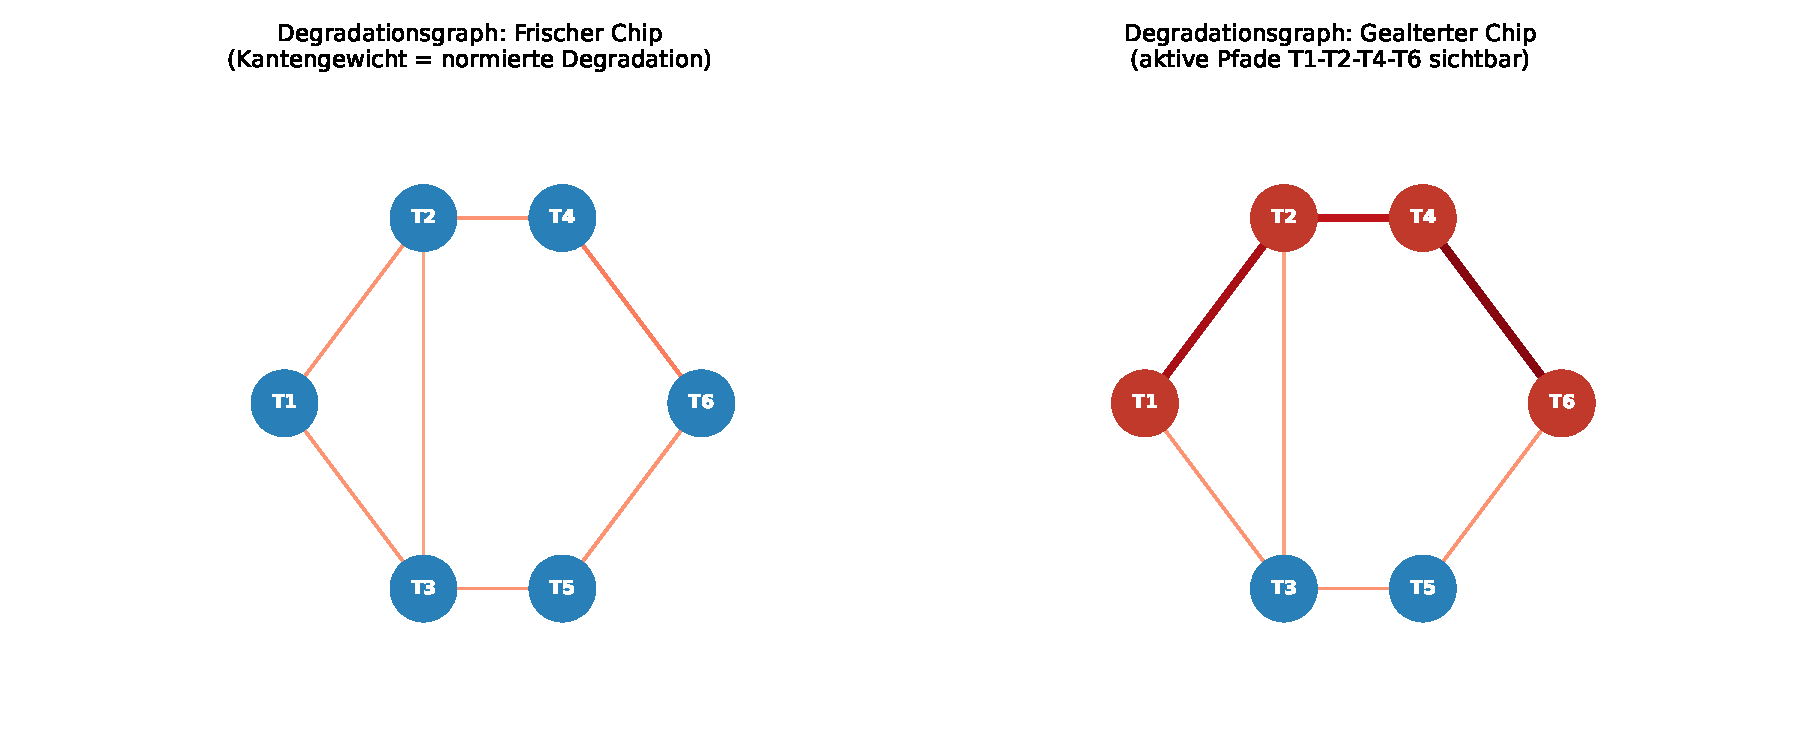
\includegraphics[width=0.92\textwidth]{plot_subgraph.pdf}
	\caption{Degradationsgraphen: Links der Graph eines frischen Chips
	(alle Kantengewichte niedrig, gleichmäßige Degradation).
	Rechts der Graph nach Betrieb: Aktive Pfade T1--T2--T4--T6
	haben deutlich höhere Kantengewichte (rot markiert).
	Der Subgraph-Vergleich beider Graphen identifiziert algorithmisch
	die aktiven Pfade als dominanten Teilgraph.}
	\label{fig:subgraph}
\end{figure}

\textbf{Degradationsgraphen.}
Ein Degradationsgraph $G_D = (V, E, w)$ ist ein gewichteter gerichteter Graph,
in dem:
\begin{itemize}
	\item jeder Knoten $v_i \in V$ einen Transistor oder eine Leitbahn repräsentiert,
	\item jede Kante $(v_i, v_j) \in E$ eine physikalische Abhängigkeit
	      (gemeinsamer Strompfad, thermische Kopplung) beschreibt,
	\item das Kantengewicht $w(v_i, v_j) \in [0,1]$ die normierte Degradation
	      der Verbindung quantifiziert.
\end{itemize}

Nach einem Betriebszyklus hat ein aktiver Pfad ein deutlich höheres Kantengewicht
als ein inaktiver Pfad. Der Subgraph Algorithmus vergleicht nun den Degradationsgraphen
$G_D^{\rm after}$ nach dem Betrieb mit dem Referenzgraphen $G_D^{\rm before}$:
\begin{itemize}
	\item Knoten und Kanten mit $w > w_{\rm threshold}$ bilden den
	      \emph{aktiven Teilgraphen} $G_D^{\rm active}$.
	\item Der Subgraph-Vergleich $G_D^{\rm active} \subseteq G_D^{\rm design}$
	      verifiziert, ob die aktivierten Pfade der Entwurfsspezifikation entsprechen.
	\item Unerwartete Teilgraphen — Pfade mit hoher Degradation, die laut Spezifikation
	      inaktiv sein sollten — weisen auf Designfehler oder unerwünschte Aktivierung
	      durch Glitches hin.
\end{itemize}

\textbf{Algorithmus zur Pfadidentifikation.}
Sei $\sigma_j^{\rm before}$ die Signatur von Spalte $j$ des Degradationsgraphen
vor dem Betrieb und $\sigma_j^{\rm after}$ danach. Die Differenz-Signatur
$\Delta\sigma_j = \sigma_j^{\rm after} - \sigma_j^{\rm before}$ ist ein
Maß für die Degradation auf Pfad $j$. Der Subgraph Algorithmus identifiziert
diejenige zyklische Rotation des Differenz-Signaturarrays, die maximale
LCS-Ãœbereinstimmung mit dem bekannten Aktivierungsmuster des Eingabevektors
ergibt. Damit reduziert sich die Pfadidentifikation auf das bekannte
Subgraph-Isomorphieproblem, das der Algorithmus in $O(n^3)$ löst.

\textbf{Fehlerdiagnose durch Subgraph-Differenz.}
Die Differenz $G_D^{\rm active} \setminus G_D^{\rm expected}$ — also der Teil
des aktiven Teilgraphen, der nicht erwartet wurde — ist der \emph{Fehlersubgraph}.
Seine Analyse gibt direkten Aufschluss über:
\begin{itemize}
	\item \emph{Glitch-Pfade:} Kurzfristige, unbeabsichtigte Aktivierungen durch
	      kombinatorische Hazards, die HCI-Schäden hinterlassen.
	\item \emph{Leakage-Pfade:} Subthreshold-Leckströme, die über lange Zeiten
	      EM-relevante Stromdichten in dünnen Leitbahnen erzeugen.
	\item \emph{Parametrische Fehler:} Pfade, deren Aktivierungsdauer systematisch
	      von der Spezifikation abweicht, z.\,B. durch Setup-Time-Verletzungen.
\end{itemize}

Diese Verbindung öffnet ein neues Forschungsfeld an der Schnittstelle von
Zuverlässigkeitsphysik und algorithmischer Graphentheorie, das sowohl für die
formale Verifikation als auch für die Failure Analysis industrieller Halbleiter
von hoher praktischer Relevanz ist.

\subsection{Quanteneffekte und post-CMOS-Zuverlässigkeit}
\label{sub:quantum}

Mit dem Vordringen in den Sub-2-nm-Bereich werden Quanteneffekte in der
Transistoralterung unvermeidlich. Tunnelströme durch das Gateoxid sind in
High-$k$-Dielektrika bereits heute relevant und stellen einen neuen,
quantenmechanischen Degradationsmechanismus dar: \emph{Trap-Assisted Tunneling}
(TAT) erzeugt Defekte nicht durch klassische Energieübertragung, sondern durch
quantenmechanisches Durchdringen der Potenzialbarriere.

Für Gateoxide mit $d_{\rm ox} < 1$\,nm (typisch bei GAA-Transistoren mit
High-$k$/Metal-Gate) gilt der direkte Tunnelstrom:
\[
J_{\rm tun} \propto \exp\!\left(-\frac{4\pi d_{\rm ox}}{h} \sqrt{2 m^* \phi_B}\right),
\]
wobei $m^*$ die effektive Tunnelmasse, $\phi_B$ die Barrierenhöhe und $h$ das
Planck'sche Wirkungsquantum sind. Die Defekterzeugungsrate durch TAT skaliert
mit $J_{\rm tun}^2$ und ist damit deutlich empfindlicher gegenüber
Betriebsspannung als klassische HCI. Eine weitere Erhöhung der Betriebsspannung
um 10\,\% kann die TAT-Degradationsrate um den Faktor 2--4 steigern.

Post-CMOS-Technologien wie Kohlenstoff-Nanoröhren-Transistoren (CNFET) oder
2D-Materialien (MoS$_2$, h-BN) zeigen völlig andere Alterungsmechanismen,
da sie keine Si--SiO$_2$-Grenzfläche besitzen. Neue Modelle werden erforderlich
sein, die die spezifischen Bindungsenergien und Defekttypen in diesen Materialien
berücksichtigen.

% ──────────────────────────────────────────────────────────────
\begin{thebibliography}{99}

\bibitem{black1969}
J.\,R. Black,
\emph{Electromigration — A Brief Survey and Some Recent Results},
IEEE Transactions on Electron Devices, Bd. 16, Nr. 4, S. 338--347, 1969.

\bibitem{takeda1983}
E. Takeda und N. Suzuki,
\emph{An Empirical Model for Device Degradation due to Hot-Carrier Injection},
IEEE Electron Device Letters, Bd. 4, Nr. 4, S. 111--113, 1983.

\bibitem{hu1985}
C. Hu, S.\,C. Tam, F.-C. Hsu, P.-K. Ko, T.-Y. Chan und K.\,W. Terrill,
\emph{Hot-Electron-Induced MOSFET Degradation — Model, Monitor, and Improvement},
IEEE Transactions on Electron Devices, Bd. 32, Nr. 2, S. 375--385, 1985.

\bibitem{alam2005}
M.\,A. Alam und S. Mahapatra,
\emph{A Comprehensive Model of PMOS NBTI Degradation},
Microelectronics Reliability, Bd. 45, Nr. 1, S. 71--81, 2005.

\bibitem{stathis2006}
J.\,H. Stathis und S. Zafar,
\emph{The Negative Bias Temperature Instability in MOS Devices: A Review},
Microelectronics Reliability, Bd. 46, Nr. 2--4, S. 270--286, 2006.

\bibitem{jedec2010}
JEDEC Solid State Technology Association,
\emph{JESD87B: Procedure for Measuring N-Channel MOSFET Hot-Carrier-Induced
Degradation Under DC Stress},
JEDEC Standard, 2010.

\bibitem{nikawa1992}
K. Nikawa,
\emph{Failure Analysis Applications of Emission Microscopy},
Proc. International Symposium for Testing and Failure Analysis, S. 151--158, 1992.

\bibitem{raissi2019}
M. Raissi, P. Perdikaris und G.\,E. Karniadakis,
\emph{Physics-Informed Neural Networks: A Deep Learning Framework for Solving
Forward and Inverse Problems Involving Nonlinear Partial Differential Equations},
Journal of Computational Physics, Bd. 378, S. 686--707, 2019.

\bibitem{epp2026}
S. Epp,
\emph{Der Subgraph Algorithmus},
Technischer Bericht, 2026.
\url{https://github.com/hjstephan86/subgraph}

\bibitem{kwiatkowska2011}
M. Kwiatkowska, G. Norman und D. Parker,
\emph{PRISM 4.0: Verification of Probabilistic Real-Time Systems},
Proc. 23rd International Conference on Computer Aided Verification (CAV),
Lecture Notes in Computer Science, Bd. 6806, S. 585--591, Springer, 2011.

\bibitem{aec2006}
Automotive Electronics Council,
\emph{AEC-Q100 Rev-H: Failure Mechanism Based Stress Test Qualification
for Integrated Circuits},
AEC Standard, 2006.

\end{thebibliography}

\end{document}

